\section{Objetivos}\label{sec:objetives}

El propósito central de este trabajo es la creación de un sistema que permita la extracción automática de documentos
de cualquier tipo y cualquier formato.

\begin{figure}[ht]
    \begin{center}
        
\includegraphics[width=\textwidth]{./chapter/1/images/chapter_1.overview}
        \caption{Esquema del funcionamiento general del sistema}
        \label{fig:chapter_1.overview}
    \end{center}
\end{figure}

Provisionalmente, hemos denominado al sistema \textit{DataMiner}.
Por lo tanto, nos referiremos a él como sistema de Extracción de información de documentos, el sistema o
\textit{DataMiner} indistintamente a lo largo de este trabajo.

Tal y como se puede ver en la figura~\ref{fig:chapter_1.overview} el funcionamiento es el siguiente:

\begin{enumerate}
    \item El sistema recibe un documento de cualquier tipo en cualquier formato.
    \item
    Si el sistema puede procesar el documento, tanto por el formato, como por el tipo de documento, genera un objeto que
    contiene la información relevante del documento recibido.
\end{enumerate}

\subsection*{Objetivos específicos}

Como este objetivo puede resultar demasiado ambicioso, el alcance de este TFG quedará limitado a los siguientes
objetivos específicos que aparecen en la figura~\ref{fig:chapter_1.specific_a}.

\begin{enumerate}
    \item
    \textbf{Requisito 1} Desarrollar un sistema capaz de convertir documentos \textit{PDF}~\cite{url_adobe_pdf}
    en documentos de texto plano que puedan ser procesados\label{req:transform_pdf_to_text}.
    \item
    Implementar dos casos de uso dentro del sistema:
    \begin{enumerate}
        \item
        \textbf{Requisito 2} Procesar contratos de arrendamiento de vivienda entre
        particulares\label{req:residence_lease_agreement}.
        \item
        \textbf{Requisito 3} Procesar contratos de compraventa de vehículo entre
        particulares\label{req:sale_and_purchase_agreement}.
    \end{enumerate}
\end{enumerate}

\begin{figure}[ht]
    \begin{center}
        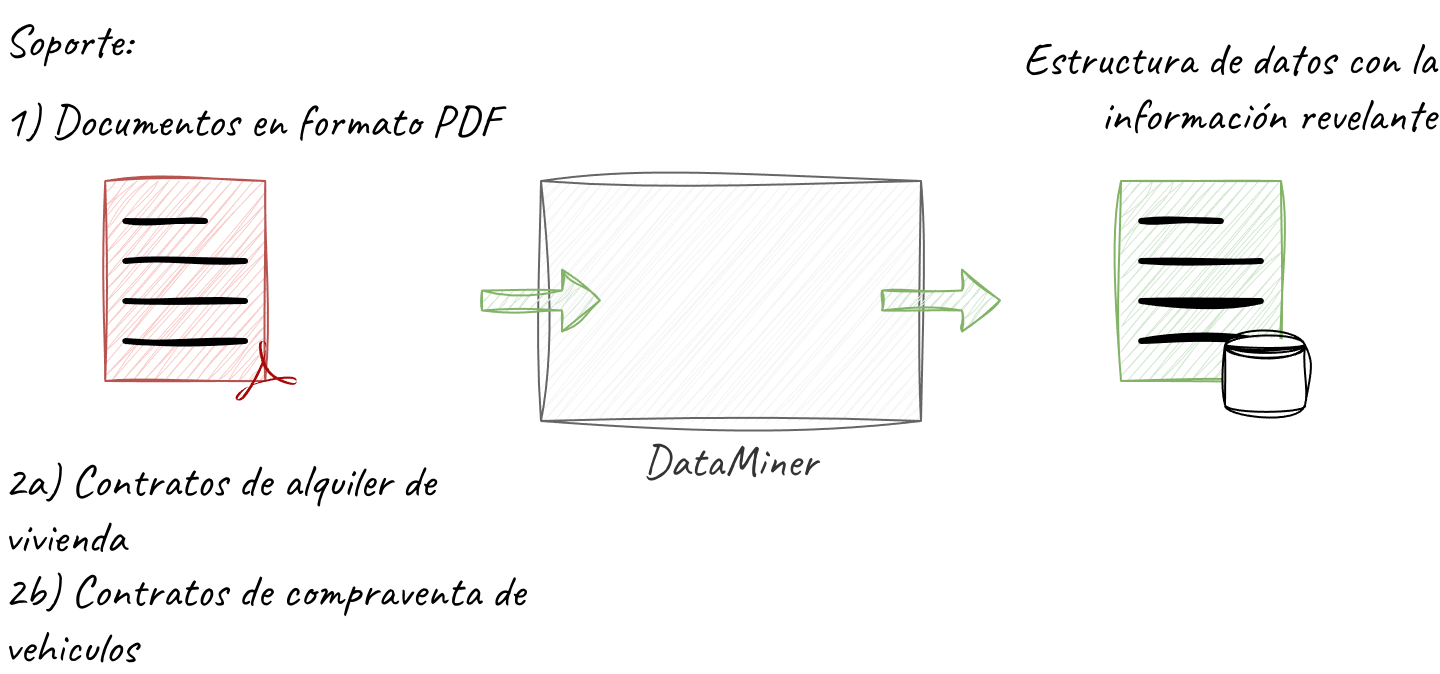
\includegraphics[width=\textwidth]{chapter/1/images/chapter_1.specific_a}
        \caption{Esquema de los objetivos específicos del TFG}
        \label{fig:chapter_1.specific_a}
    \end{center}
\end{figure}

Además, tal como aparece en la figura~\ref{fig:chapter_1.specific_b} vamos a necesitar dos elementos adicionales para
completar este trabajo.

\begin{enumerate}
    \item Desarrollar un conjunto de pruebas, que permita realizar las pruebas oportunas durante el desarrollo del
    proyecto, y que en su conclusión nos permite evaluar cuán preciso es el sistema.
    \item Desarrollar interfaces que permitan comunicarse con el sistema:
    \begin{enumerate}
        \item  Una interfaz web
        \item  Una interfaz de línea de comandos
    \end{enumerate}
\end{enumerate}

\begin{figure}[ht]
    \begin{center}
        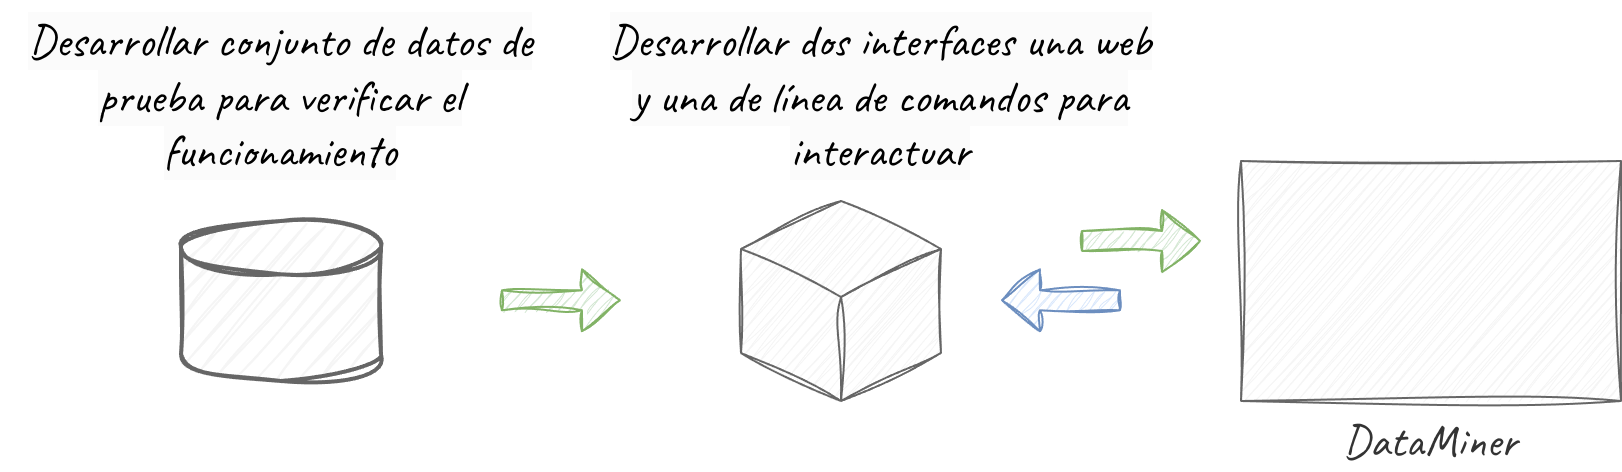
\includegraphics[width=\textwidth]{chapter/1/images/chapter_1.specific_b}
        \caption{Esquema de los conjuntos de datos prueba e interfaces interactuando con el sistema}
        \label{fig:chapter_1.specific_b}
    \end{center}
\end{figure}

Además, el sistema estará diseñado para introducir nuevas características de una forma sencilla.
Por ejemplo estas son algunas características que pueden ser añadidas fácilmente.

\begin{enumerate}
    \item
    Procesar nuevos tipos de documentos, como por ejemplo formatos de office como microsoft word o microsoft excel,
    o formatos de video o audio, etc.
    \item
    Procesar nuevos tipos de documentos, como documentos de identidad, acuerdos de confidencialidad, documentos
    de impuestos, etc.
\end{enumerate}